%\input{Preamble.tex}
\documentclass[5pt,twocolumn]{article}
\usepackage{amsmath,amssymb,amsthm}
\usepackage[left=.25truein, right=.25truein, top=.25truein, bottom=.25truein]{geometry}
\usepackage{multicol}
\usepackage{graphicx}
\makeatletter
\newcommand*\bigcdot{\mathpalette\bigcdot@{.5}}
\newcommand*\bigcdot@[2]{\mathbin{\vcenter{\hbox{\scalebox{#2}{$\m@th#1\bullet$}}}}}
\makeatother
\graphicspath{ {images/} }
\linespread{.8}
\begin{document}
	\noindent \textbf{Basic Statistics and Linear Algebra}\\
	Mean as matrix multiplication: $\mathbf{\overline{X}} = \frac{1}{n}\mathbf{X'1} = (\mathbf{X}_1 + \cdots + \mathbf{X}_n)/n$\\
	Variance as matrix multiplication: $\mathbf{S} = \frac{1}{n-1}\mathbf{X'}\left(\mathbf{I} - \frac{1}{n}\mathbf{11'}\right)\mathbf{X} = \frac{1}{n-1}\Sigma_{j=1}^n (\mathbf{X}_j - \mathbf{\overline{X}})(\mathbf{X}_j - \mathbf{\overline{X}})'$\\
	A matrix $\mathbf{A}$ is positive definite if $0 < \mathbf{x'Ax} \; \forall \mathbf{x} \neq \mathbf{0}$\\
	If two vectors have angle $\theta$ between them, then $\cos(\theta) = \frac{\mathbf{x'y}}{\sqrt{\mathbf{x'x}}\sqrt{\mathbf{y'y}}}$\\
	Transpose of a matrix: first row becomes first column (with entries in same order)\\
	Matrix multiplication: take dot product of row with column\\
	If $\mathbf{A} = \begin{bmatrix}
a & b\\
c & d
\end{bmatrix}$, then $|\mathbf{A}| = ad - bc$\\
	\indent If $\mathbf{A} = \begin{bmatrix}
a & b & c\\
d & e & f\\
g & h & i
\end{bmatrix}$ is 3x3, then \\
	\indent \indent $|\mathbf{A}| = a \cdot \begin{vmatrix}
e & f\\
h & i
\end{vmatrix} - b \cdot \begin{vmatrix}
d & f\\
g & i
\end{vmatrix} + c \cdot \begin{vmatrix}
d & e\\
g & h
\end{vmatrix}$\\
	\indent The pattern of alternating + and - holds for larger matrices.\\
	\textbf{Finding eigenvalues:} $|\mathbf{A} - (\lambda \cdot \mathbf{I})|$\\
	\textbf{Finding eigenvectors:} $(\mathbf{A} - \lambda_i) \cdot \mathbf{e}_i = \mathbf{0}$\\
	If $\mathbf{A} = \begin{bmatrix}
a & b\\
c & d
\end{bmatrix}$, then $\mathbf{A}^{-1} = \frac{1}{ad - bc}\begin{bmatrix}
d & -b\\
-c & a
\end{bmatrix}$\\
	\noindent \textbf{Ch. 5 - Inferences About a Mean Vector}\\
	\textbf{Hotelling's $T^2$:} Tests for plausibility of multivariate mean vector\\
	\indent $T^2 = n(\mathbf{\overline{X}} - \mathbf{\mu}_0)'\left(\mathbf{S}\right)^{-1}(\mathbf{\overline{X}} - \mathbf{\mu}_0) \sim \frac{(n-1)p}{n-p}F_{p, n-p}$\\
	\indent Reject $\text{H}_0: \mathbf{\mu} = \mathbf{\mu_0}$ vs. $\text{H}_1: \mathbf{\mu} \neq \mathbf{\mu_0}$ at the level $\alpha$ of significance if $T^2 > \frac{(n-1)p}{n-p}F_{p, n-p}(\alpha)$\\
	\indent $T^2$is invariant under changes in units of measurements for $\mathbf{X}$ of the form $\mathbf{Y} = \mathbf{C}\mathbf{X} + \mathbf{d}$, $\mathbf{C}$ nonsingular.\\
	\textbf{Confidence region for mean:} $n(\mathbf{\overline{X}} - \mathbf{\mu})'\left(\mathbf{S}\right)^{-1}(\mathbf{\overline{X}} - \mathbf{\mu}) \leq \frac{(n-1)p}{n-p}F_{p, n-p}(\alpha)$\\
	\indent For 2 dimensional case, the center of the ellipse is at $\mathbf{\overline{x}}$. \\
	\indent Next find the eignevalues and eigenvectors for $\mathbf{S}$.\\
	\indent Half lengths of the major and minor axes of the ellipse are given by $\sqrt{\lambda_i}\sqrt{\frac{(n-1)p}{n-p}F_{p, n-p}(\alpha)}$ for each $i$\\
	\indent The axes lie along the eigenvectors $\mathbf{e}_i$ when they are plotted with $\mathbf{\overline{x}}$ as the origin\\
	\textbf{One-at-a-time confidence statements:}\\
	\indent $\overline{x}_i - t_{n-1}(\alpha/2)\sqrt{\frac{s_{ii}}{n}} \leq \mu_i \leq \overline{x}_i + t_{n-1}(\alpha/2)\sqrt{\frac{s_{ii}}{n}}$\\
	\textbf{Simultaneous confidence statements:}\\
	\indent $\left(\mathbf{a}'\mathbf{\overline{X}} - \sqrt{\frac{(n-1)p}{n-p}F_{p, n-p}(\alpha)\mathbf{a'Sa}}, \mathbf{a}'\mathbf{\overline{X}} + \sqrt{\frac{(n-1)p}{n-p}F_{p, n-p}(\alpha)\mathbf{a'Sa}}\right)$ \\
	\indent will contain $\mathbf{a'\mu}$ with probability $1 - \alpha$.\\
	\textbf{Bonferroni method of multiple comparisons:}\\
	\indent $\overline{x}_i - t_{n-1}\left(\frac{\alpha}{2p}\right)\sqrt{\frac{s_{ii}}{n}} \leq \mu_i \leq \overline{x}_i + t_{n-1}\left(\frac{\alpha}{2p}\right)\sqrt{\frac{s_{ii}}{n}}$\\
	\textbf{Large Sample Mean Inference:} If $n-p$ large, then $\mathbf{a'\overline{X}} \pm \sqrt{\chi_p^2(\alpha)}\sqrt{\frac{\mathbf{a'Sa}}{n}}$  will contain $\mathbf{a'\mu}$ for every $\mathbf{a}$ with probability $1 - \alpha$.\\
	\textbf{EM algorithm for missing data:} Let $\mathbf{T_1} = \Sigma_{j=1}^n \mathbf{X_j} = n\mathbf{\overline{X}}$ and $\mathbf{T_2} = \Sigma_{j=1}^n \mathbf{X}_j \mathbf{X}_j' = (n-1)S + n \mathbf{\overline{X}\overline{X}}'$\\
	\indent \textbf{Estimation step:} Compute the revised maximum likelihood estimates $\mathbf{\tilde{\mu}} = \frac{\mathbf{\widetilde{T}_1}}{n}$, $\mathbf{\tilde{\Sigma}} = \frac{1}{n}\widetilde{\mathbf{T}}_2 - \mathbf{\tilde{\mu}}\mathbf{\tilde{\mu}'}$\\
	\indent \textbf{Prediction step:} For each vector $\mathbf{x_j}$ with missing values, let $\mathbf{x_j}^{(1)}$ denote the missing components and $\mathbf{x_j}^{(2)}$ denote those components which are available. Thus, $\mathbf{x_j}' = \begin{bmatrix}
\mathbf{x_j}^{(1)'} & \mathbf{x_j}^{(2)'}\\
\end{bmatrix}$\\
	\indent Now, $\mathbf{\tilde{x}}_j^{(1)} = \mathbf{\tilde{\mu}}^{(1)} + \mathbf{\tilde{\Sigma}}_{12}\mathbf{\tilde{\Sigma}}_{22}^{-1}(\mathbf{x}_j^{(2)} - \mathbf{\tilde{\mu}}^{(2)})$\\
	\indent $\widetilde{\mathbf{x}_j^{(1)}\mathbf{x}_j^{(1)'}} = \mathbf{\tilde{\Sigma}}_{11} - \mathbf{\tilde{\Sigma}}_{12}\mathbf{\tilde{\Sigma}}_{22}^{-1}\mathbf{\tilde{\Sigma}}_{21} + \mathbf{\tilde{x}}_j^{(1)}\mathbf{\tilde{x}}_j^{(1)'}$\\
	\indent $\widetilde{\mathbf{x}_j^{(1)}\mathbf{x}_j^{(2)'}} = \mathbf{\tilde{x}}_j^{(1)}\mathbf{x}_j^{(2)'}$\\
	Now repeat estimation step using the predicted data.\\
	\noindent \textbf{Ch. 6 - Comparisons of Several Multivariate Means}\\
	\textbf{Comparing mean vectors from two populations:}\\
	\indent $\mathbf{S}_{pooled} = \frac{n_1 - 1}{n_1 + n_2 - 2}\mathbf{S_1} + \frac{n_2 - 1}{n_1 + n_2 - 2}S_2$
	\indent $T^2 = [\mathbf{\overline{X}_1} - \mathbf{\overline{X}_2} - (\mathbf{\mu}_1 - \mathbf{\mu}_2)]'\left[\left(\frac{1}{n_1} + \frac{1}{n_2}\right)\mathbf{S}_{pooled}\right]^{-1}[\mathbf{\overline{X}_1} - \mathbf{\overline{X}_2} - (\mathbf{\mu}_1 - \mathbf{\mu}_2)] \sim \frac{(n_1 + n_2 - 2)p}{(n_1 + n_2 - p - 1)}F_{p, n_1 + n_2 - p - 1}$\\
	\indent So reject $\text{H}_0: \mathbf{\mu}_1 - \mathbf{\mu}_2 = \mathbf{\delta}_0$ if\\
	\indent $T^2 > c^2 = \frac{(n_1 + n_2 - 2)p}{(n_1 + n_2 - p - 1)}F_{p, n_1 + n_2 - p - 1}$\\
	\textbf{Simultaneous confidence intervals:} Using same $c^2$ as above, with probability $1 - \alpha$,\\
	\indent $\mathbf{a}'(\mathbf{\overline{X}}_1 - \mathbf{\overline{X}}_2) \pm c \sqrt{\mathbf{a}'\left(\frac{1}{n_1} + \frac{1}{n_2}\right)\mathbf{S}_{pooled}\mathbf{a}}$\\
	\indent will cover $\mathbf{a}'(\mathbf{\mu}_1 - \mathbf{\mu}_2)$ for all $\mathbf{a}$\\
	\textbf{Two-sample situation when $\Sigma_1 \neq \Sigma_2$:}\\
	\indent Let the sample sizes be such that $n_1 - p$ and $n_2 - p$ are large.\\
	\indent Then an approximate $100(1 - \alpha)$\% confidence ellipsoid for\\
	\indent $\mathbf{\mu}_1 - \mathbf{\mu}_2$ is given by all $\mu_1 - \mu_2$ satisfying\\
	\indent $[\mathbf{\overline{x}}_1 - \mathbf{\overline{x}}_2 - (\mathbf{\mu}_1 - \mathbf{\mu}_2)]'\left[\frac{1}{n_1}\mathbf{S}_1 + \frac{1}{n_2}\mathbf{S}_2\right]^{-1}[\mathbf{\overline{x}}_1 - \mathbf{\overline{x}}_2 - (\mathbf{\mu}_1 - \mathbf{\mu}_2)] \leq \chi^2_p(\alpha)$\\
	\textbf{One-way MANOVA:} $\mathbf{X}_{\ell j} = \mathbf{\mu} + \mathbf{\tau}_{\ell} + \mathbf{e}_{\ell j}$ with $j = 1, 2, \cdots, n_{\ell}$ and $\ell = 1, 2, \cdots, g$\\
	\indent $\mathbf{\mu}$ is overall mean, $\mathbf{\tau}_{\ell}$ represents the $\ell$th treatment effect. $\mathbf{e}_{\ell j}$ are independent $N_p(\mathbf{0}, \mathbf{\Sigma})$.\\
	\indent A vector of observations may be decomposed as suggested by model. Thus,
	$\mathbf{x}_{\ell j} = \mathbf{\overline{x}} + (\mathbf{\overline{x}}_{\ell} - \mathbf{\overline{x}}) + (\mathbf{x}_{\ell j} - \mathbf{\overline{x}}_{\ell})$
	which is\\
	\indent observation = overall sample mean $(\hat{\mathbf{\mu}})$ + estimated treatment effect ($\hat{\mathbf{\tau}}_{\ell})$ + residual $(\hat{\mathbf{e}}_{\ell j})$\\
	The MANOVA table to for comparing population mean vectors is given by\\
	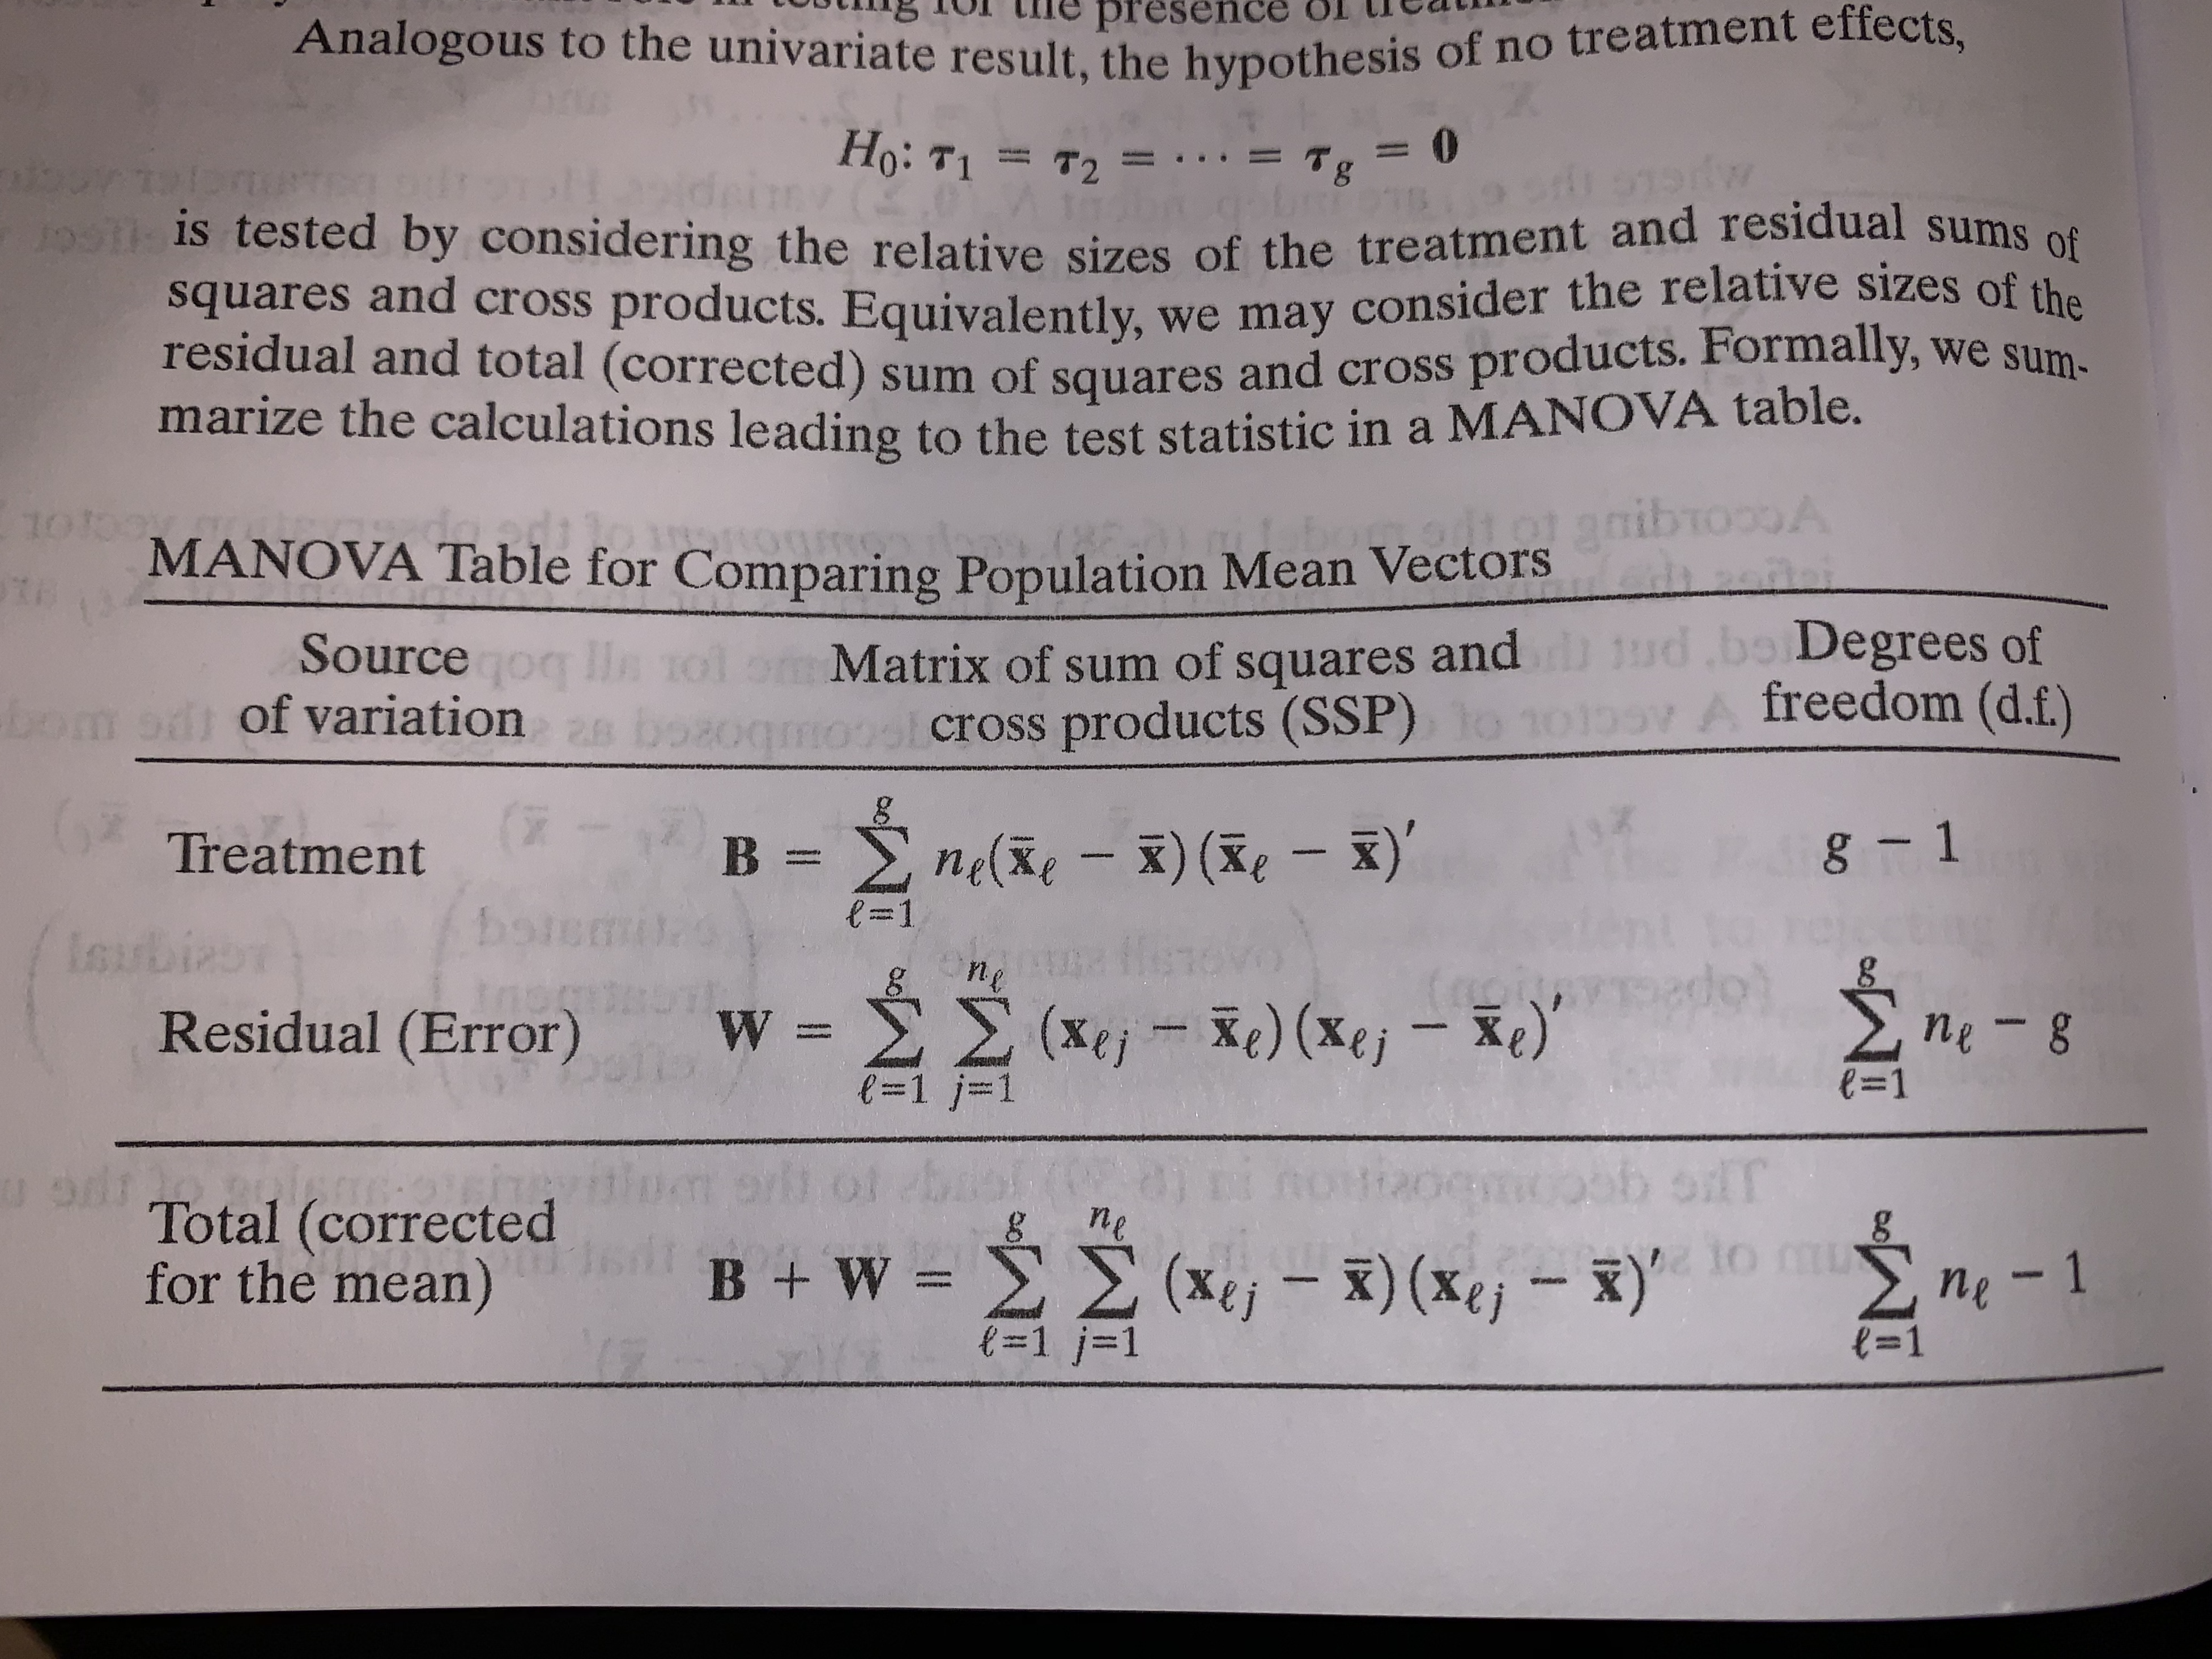
\includegraphics[scale=0.075]{IMG_0491}\\
	One test for $\text{H}_0: \mathbf{\tau}_1 = \mathbf{\tau}_2 = \cdots = \mathbf{\tau}_g = \mathbf{0}$ (ie. no treatment effect). Called \textit{Wilks' lambda}.\\
	The exact distribution for Wilks' lambda is given for special cases in the following table:\\
	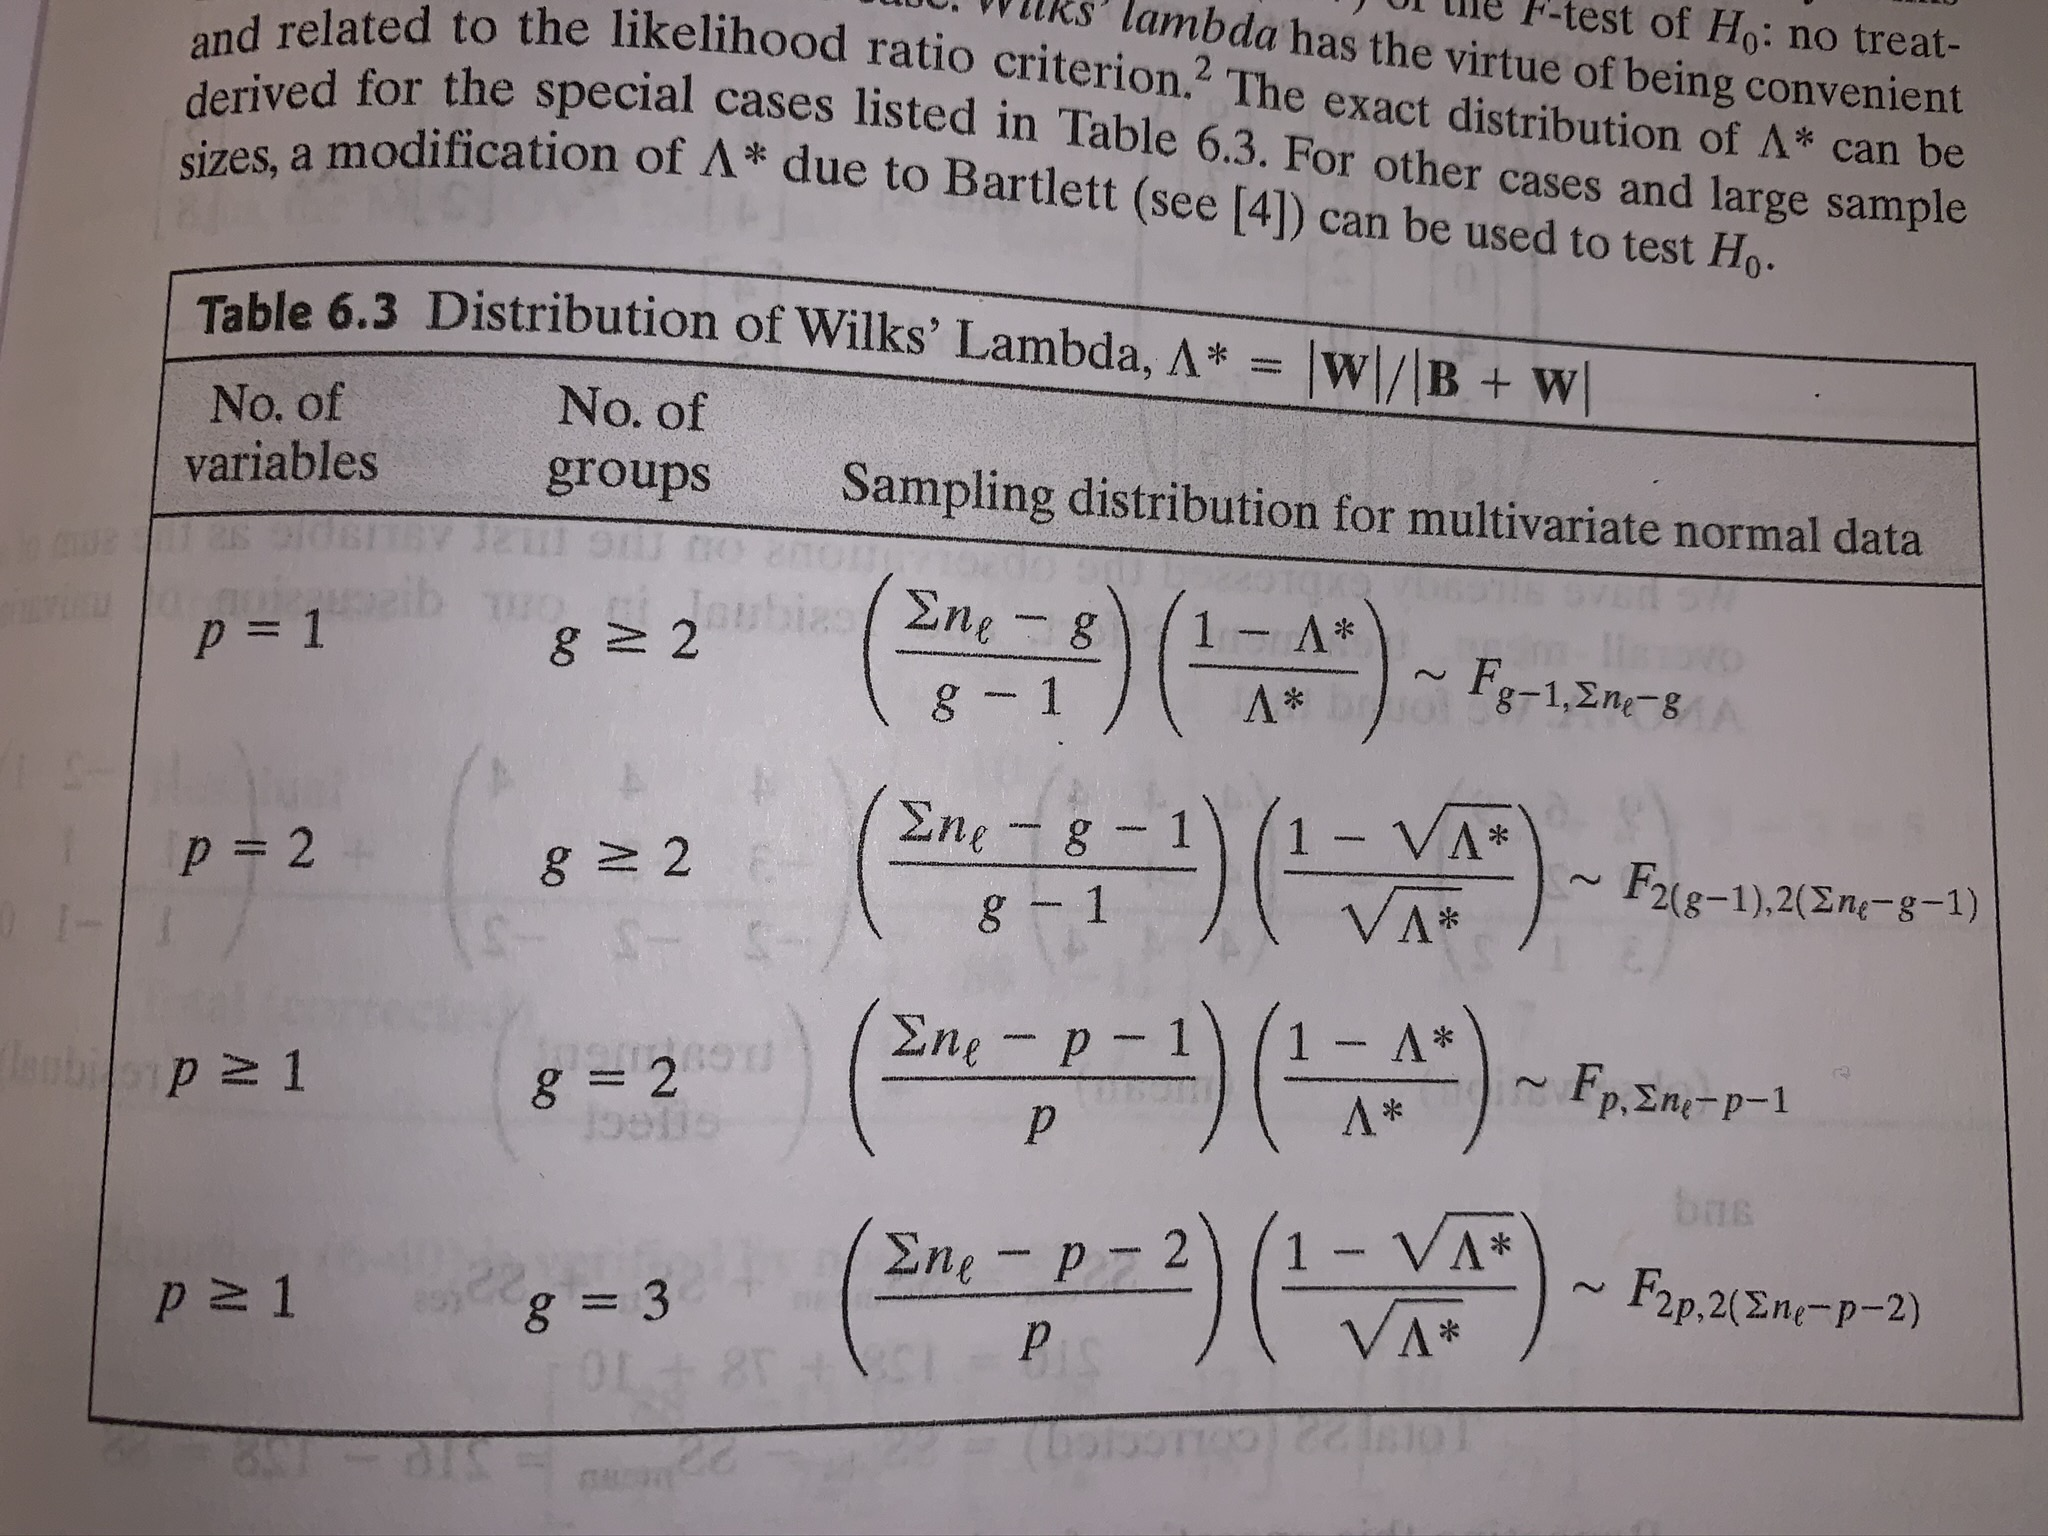
\includegraphics[scale=0.12]{IMG_0495}\\
	\newpage
	\textbf{Simultaneous confidence intervals for treatment effects:} 
	\indent Let $n = \Sigma_{k=1}^g n-k$. For the MANOVA model above, with confidence at least $(1 - \alpha)$, $\tau_{ki} - \tau_{\ell i}$ belongs to\\
	\indent $\overline{x}_{ki} - \overline{x}_{ki} \pm t_{n-g}\left(\frac{\alpha}{pg(g - 1)}\right)\sqrt{\frac{w_{ii}}{n - g}\left(\frac{1}{n_k} + \frac{1}{n_{\ell}}\right)}$\\
	\indent where $w_{ii}$ is the ith diagonal element of $\mathbf{W}$ from the MANOVA table\\
	\textbf{Two-way MANOVA:} We specify the two-way fixed-effects model for a \textit{vector} response consisting of $p$ components\\
	\indent $\mathbf{X}_{\ell k r} = \mathbf{\mu} + \mathbf{\tau}_{\ell} + \mathbf{\beta}_k + \mathbf{\gamma}_{\ell k} + \mathbf{e}_{\ell k r}$ with $\ell = 1, 2, \cdots, g$, $k = 1, 2, \cdots, b$, $r = 1, 2, \cdots, n$, where,\\
	\indent $\Sigma_{\ell = 1}^g \mathbf{\tau}_{\ell} = \Sigma_{k=1}^b \mathbf{\beta}_k = \Sigma_{\ell = 1}^g \mathbf{\gamma}_{\ell k} = \Sigma_{k = 1}^b \mathbf{\gamma}_{\ell k} = \mathbf{0}$\\
	\indent The vectors are all of order $p \times 1$ and the $\mathbf{e}_{\ell k r}$ are independent $N_p(\mathbf{0}, \mathbf{\Sigma})$\\
	\indent We can decompose the observation vectors $\mathbf{x}_{\ell kr}$ as\\
	\indent $\mathbf{x}_{\ell k r} = \mathbf{\overline{x}} + (\mathbf{\overline{x}}_{\ell \bigcdot} - \mathbf{\overline{x}}) + (\mathbf{\overline{x}}_{\bigcdot k} - \mathbf{\overline{x}}) + (\mathbf{\overline{x}}_{\ell k} - \mathbf{\overline{x}}_{\ell \bigcdot} - \mathbf{\overline{x}}_{\bigcdot k} + \mathbf{\overline{x}}) + (\mathbf{x}_{\ell k r} - \mathbf{\overline{x}}_{\ell k})$\\
	\indent where $\mathbf{\overline{x}}$ is the overall average of the observation vectors, $\mathbf{\overline{x}}_{\ell \bigcdot}$ is the average of the observation vectors at the $\ell$th level of factor 1, $\mathbf{\overline{x}}_{\bigcdot k}$ is the average of the observation vectors at the $k$th level of factors 2, $\mathbf{\overline{x}}_{\ell k}$ is the average of the observation vectors at the $\ell$th level of factor 1 \textit{and} the $k$th level of factor 2.\\
	The MANOVA table for comparing factors and their interactions is the following:\\
	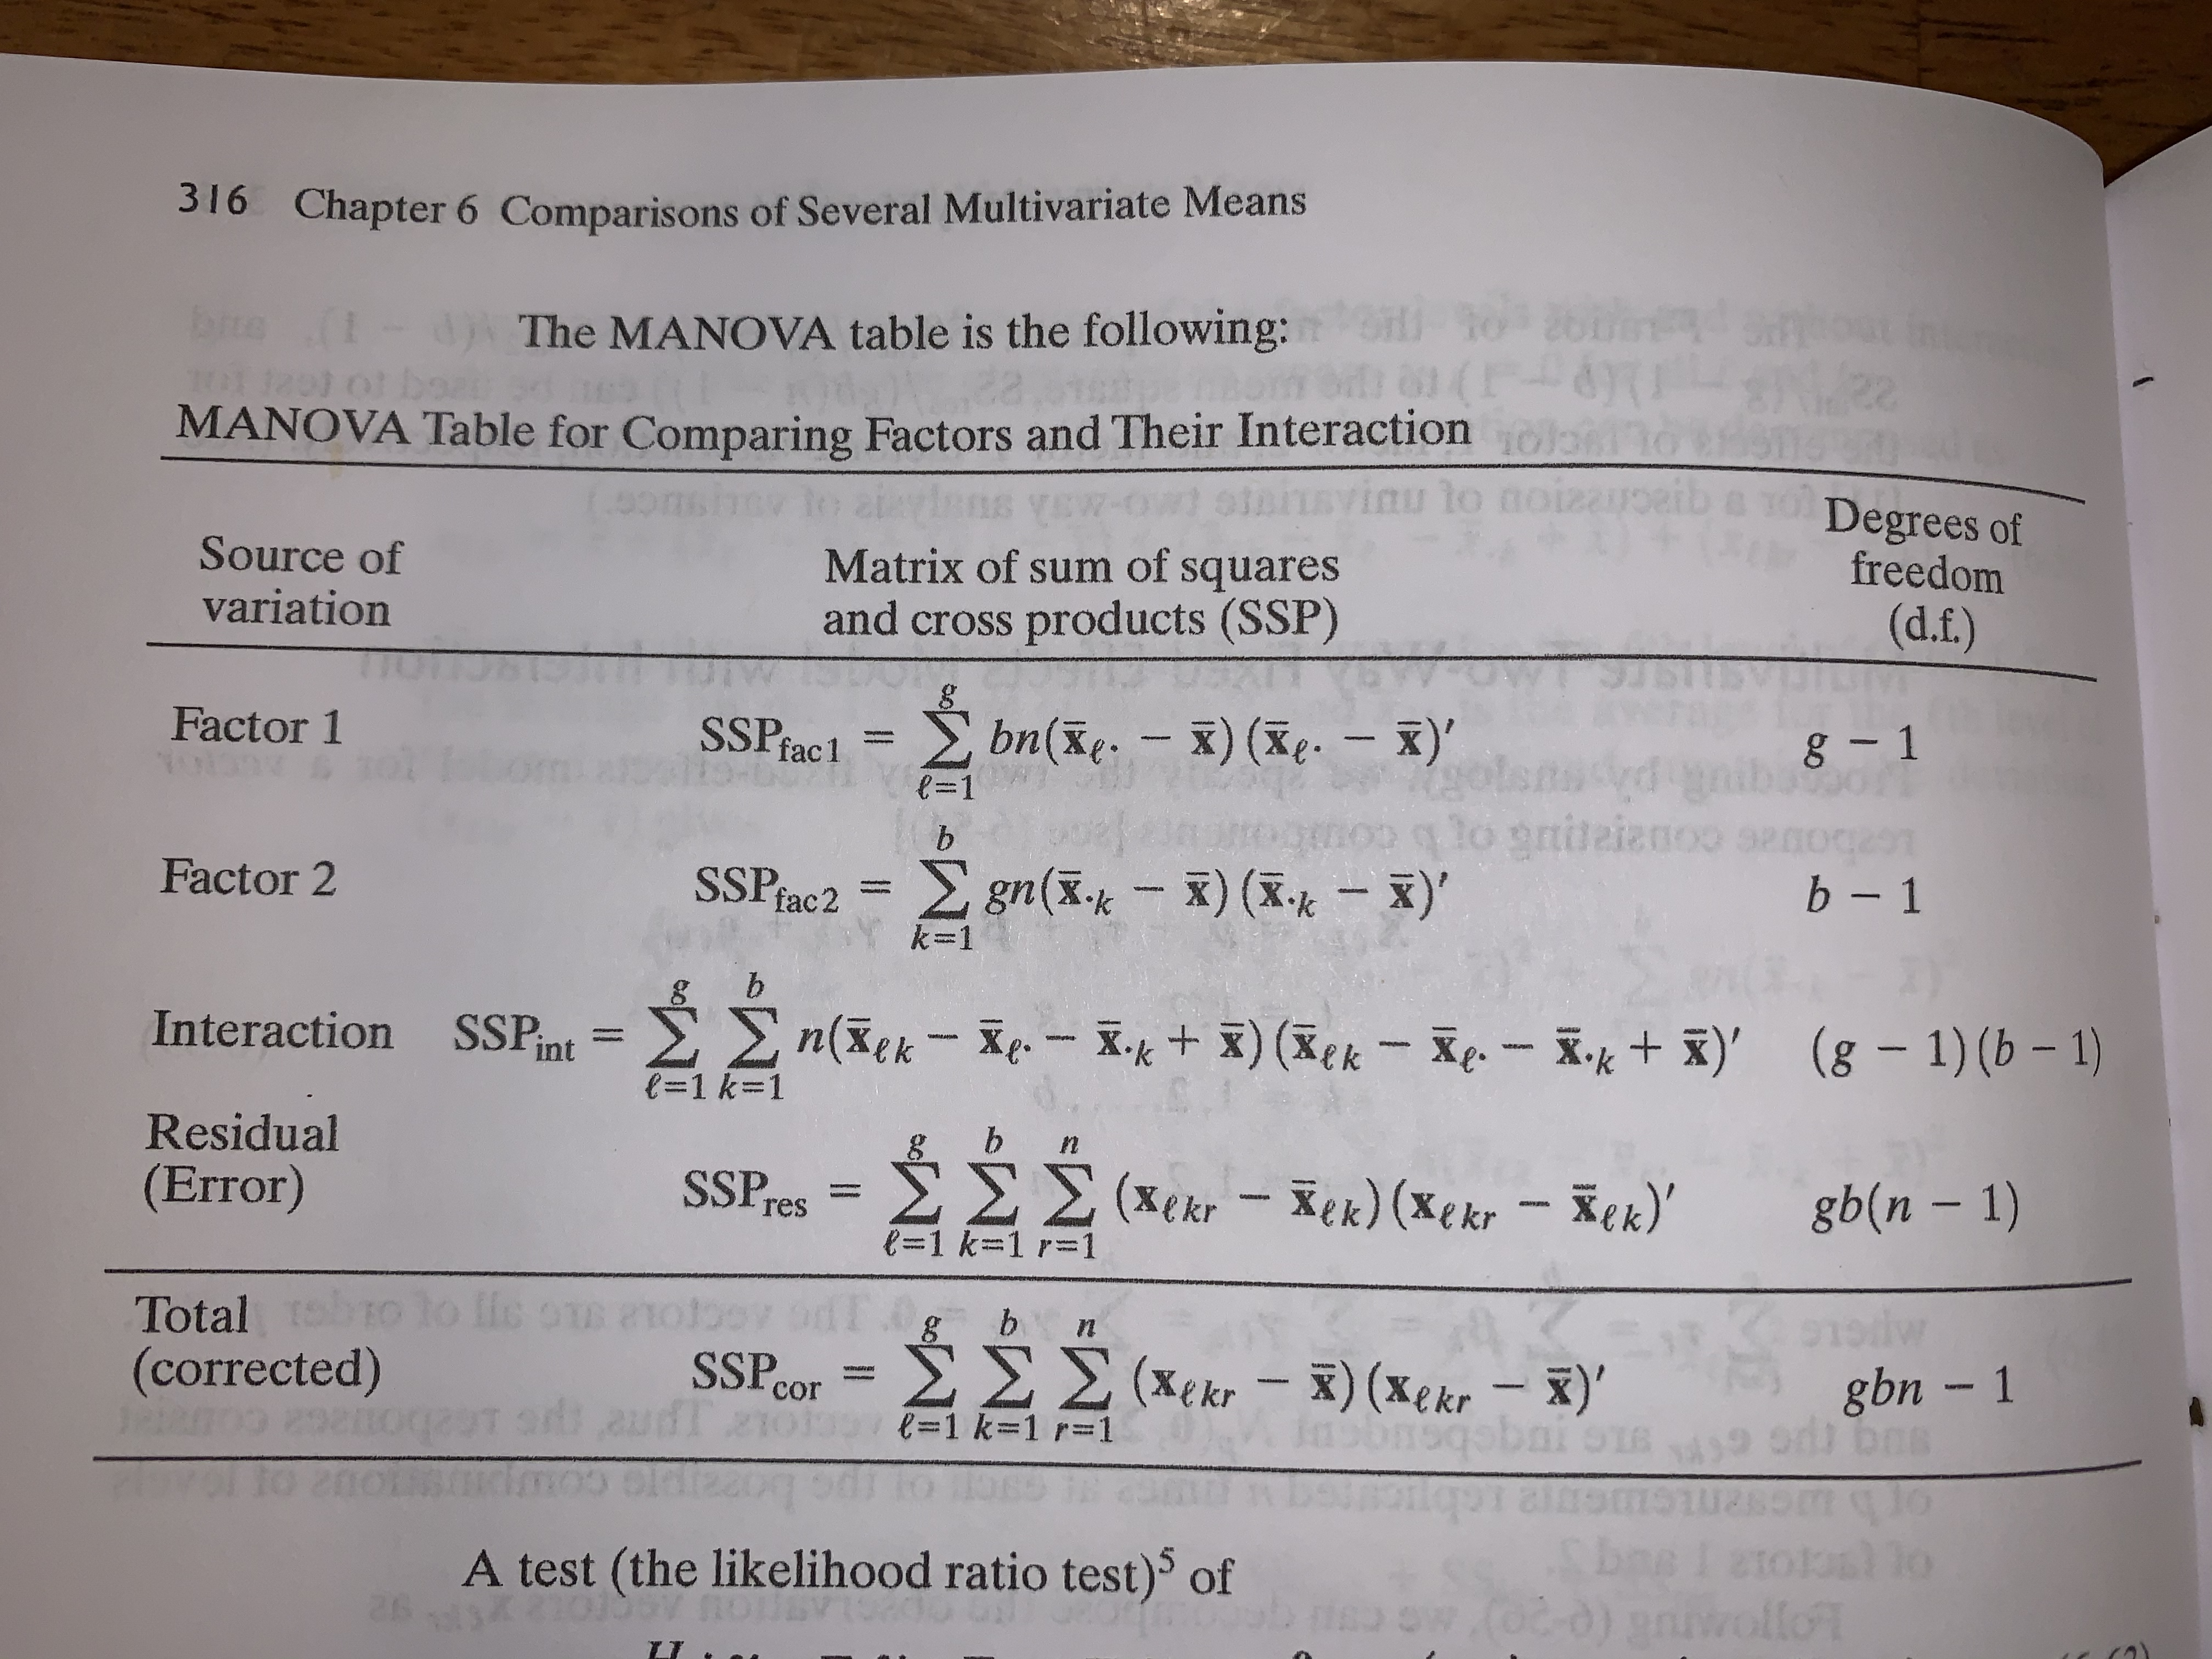
\includegraphics[scale=0.07]{IMG_0493}\\
	A test of $\text{H}_0: \mathbf{\gamma}_{11} = \mathbf{\gamma}_{12} = \cdots = \mathbf{\gamma}_{gb} = \mathbf{0}$ (ie. no interaction effects) vs. $\text{H}_1:$ at least one $\mathbf{\gamma}_{\ell k} \neq \mathbf{0}$ is conducted by rejecting $\text{H}_0$ for small values of the ratio $\Lambda^* = \frac{|\text{SSP}_{\text{res}}|}{|\text{SSP}_{\text{int}} + \text{SSP}_{\text{res}}|}$\\
	\indent Reject $\text{H}_0$ as above at the $\alpha$ level if\\
	\indent $-\left[gb(n-1) - \frac{p + 1 - (g - 1)(b - 1)}{2}\right]\ln\Lambda^* > \chi^2_{(g-1)(b-1)p}(\alpha)$\\
	Now test for factor 1 main effects. Let $\text{H}_0 = \mathbf{\tau}_1 = \mathbf{\tau}_2 = \cdots = \mathbf{\tau}_g = \mathbf{0}$ and $\text{H}_1:$ at least one $\mathbf{\tau}_{\ell} \neq \mathbf{0}$. Let,\\
	\indent $\Lambda^* = \frac{|\text{SSP}_{\text{res}}|}{|\text{SSP}_{\text{fac1}} + \text{SSP}_{\text{res}}|}$\\
	\indent Reject $\text{H}_0$ at the level $\alpha$ if\\
	\indent $-\left[gb(n-1) - \frac{p + 1 - (g - 1)}{2}\right]\ln\Lambda^* > \chi^2_{(g-1)p}(\alpha)$\\
	Lastly, factor 2 effects are tested by considering $\text{H}_0: \mathbf{\beta}_1 = \mathbf{\beta}_2 = \cdots = \mathbf{\beta}_b = \mathbf{0}$ and $\text{H}_1:$ at least one $\mathbf{\beta}_k \neq \mathbf{0}$. Let,\\
	\indent $\Lambda^* = \frac{|\text{SSP}_{\text{res}}|}{|\text{SSP}_{\text{fac2}} + \text{SSP}_{\text{res}}|}$\\
	\indent Reject $\text{H}_0$ at the level $\alpha$ if\\
	\indent $-\left[gb(n-1) - \frac{p + 1 - (b - 1)}{2}\right]\ln\Lambda^* > \chi^2_{(b-1)p}(\alpha)$\\
	The $100(1 - \alpha)$\% simultaneous confidence intervals for $\tau_{\ell i} - \tau_{mi}$ are $\tau_{\ell i} - \tau_{mi}$ belongs to $(\overline{x}_{\ell \bigcdot i} - \overline{x}_{m \bigcdot i} \pm t_v\left(\frac{\alpha}{pg(g - 1)}\right)\sqrt{\frac{E_{ii}}{v}\frac{2}{bn}}$\\
	\indent where $v = gb(n-1)$, $E_{ii}$ is the $i$th diagonal element of $\mathbf{E} = \text{SSP}_{\text{res}}$, and $\overline{x}_{\ell \bigcdot i} - \overline{x}_{m \bigcdot i}$ is the $i$th component of $\mathbf{\overline{x}}_{\ell \bigcdot} - \mathbf{\overline{x}}_{m \bigcdot}$\\
	Similarly, the $100(1-\alpha)$\% simultaneous confidence intervals for $\beta_{ki} - \beta_{qi}$ are $\beta_{ki} - \beta_{qi}$ belongs to $(\overline{x}_{\bigcdot ki} - \overline{x}_{\bigcdot qi} \pm t_v\left(\frac{\alpha}{pb(b - 1)}\right)\sqrt{\frac{E_{ii}}{v}\frac{2}{gn}}$\\
	\indent where $v$ and $E_{ii}$ are as just defined and $\overline{x}_{\bigcdot ki} - \overline{x}_{\bigcdot qi}$ is the $i$th component of $\mathbf{\overline{x}}_{\bigcdot k} - \mathbf{\overline{x}}_{\bigcdot q}$\\
	\textit{Comment}: We have considered the multivariate two-way model with replications. That is, the model allows for $n$ replications of the responses at each combination of factor levels. This enables us to examine the ''interaction`` of the factors. If only one observation vector is available at each combination of factor levels, the two-way model does not allow for the possibility of a general interaction term $\mathbf{\gamma}_{\ell k}$. The corresponding MANOVA table includes only factor 1, factor 2, and residual sources of variation as components of the total variation.\\
	\noindent \textbf{Ch. 7 - Multivariate Linear Regression Models}\\
	Classical linear regression model: $\mathbf{Y} = \mathbf{Z}\mathbf{\beta} + \mathbf{\epsilon}$ with $\mathbf{Y}$ having dimension $(n \times 1)$, $\mathbf{Z}$ $(n \times (r+1))$, and $\mathbf{\epsilon}$ $(n \times 1)$.\\
	\indent In addition, $E(\mathbf{\epsilon}) = \mathbf{0}$ $[\text{size} (n \times 1)]$ and Cov$(\mathbf{\epsilon}) = \sigma^2\mathbf{I}$ $[\text{size} (n \times n)]$\\
	\textbf{Method of least squares:} selects $\mathbf{b}$ so as to minimize the sum of the squares of the differences: $S(\mathbf{b}) = \Sigma_{j=1}^n (y_j - b_0 - b_1z_{j1} - \cdots - b_r z_{jr})^2 = (\mathbf{y} - \mathbf{Zb})'(\mathbf{y} - \mathbf{Zb})$\\
	\indent Least squares estimate of $\mathbf{\beta}:$ $\mathbf{\hat{\beta}} = (\mathbf{Z}'\mathbf{Z})^{-1}\mathbf{Z}'\mathbf{y}$\\
	$\mathbf{\hat{y}} = \mathbf{Z\hat{\beta}} = \mathbf{Hy}$ denotes the fitted values of $\mathbf{y}$, where $\mathbf{H} = \mathbf{Z}(\mathbf{Z'Z})^{-1}\mathbf{Z'}$\\
	The \textbf{residuals} are $\mathbf{\hat{\epsilon}} = \mathbf{y} - \mathbf{\hat{y}} = [\mathbf{I} - \mathbf{Z}(\mathbf{Z'Z})^{-1}\mathbf{Z'}]\mathbf{y} = (\mathbf{I} - \mathbf{H})\mathbf{y}$\\
	\indent and satisfy $\mathbf{Z'\hat{\epsilon}} = \mathbf{0}$ and $\mathbf{\hat{y}'\hat{\epsilon}} = 0$.\\
	Also, the \textbf{residual sum of squares} $= \mathbf{\hat{\epsilon}'\hat{\epsilon}} = \mathbf{y}'[\mathbf{I} - \mathbf{Z}(\mathbf{Z'Z})^{-1}\mathbf{Z'}]\mathbf{y} = \mathbf{y}'\mathbf{y} - \mathbf{y'Z\hat{\beta}}$\\
	\textbf{Sum of squares decomposition:} $\Sigma_{j=1}^n (y_j - \overline{y})^2 = \Sigma_{j=1}^n (\hat{y}_j - \overline{y})^2 + \Sigma_{j=1}^n \hat{\epsilon}_j^2$\\
	Under the general linear regression model, the least squares estimator $\mathbf{\hat{\beta}}$ has $E(\mathbf{\hat{\beta}}) = \mathbf{\beta}$ and Cov$(\mathbf{\hat{\beta}}) = \sigma^2(\mathbf{Z}'\mathbf{Z})^{-1}$.\\
	\indent $E(\mathbf{\hat{\epsilon}}) = \mathbf{0}$ and Cov$(\mathbf{\hat{\epsilon}}) = \sigma^2[\mathbf{I} - \mathbf{H}]$\\
	\textbf{Confidence region for $\mathbf{\beta}$:} $100(1-\alpha)$\% confidence region for $\mathbf{\beta}$ given by\\
	\indent $(\mathbf{\beta} - \mathbf{\hat{\beta}})'\mathbf{Z'Z}(\mathbf{\beta} - \mathbf{\hat{\beta}}) \leq (r+1)s^2F_{r+1, n-r-1}(\alpha)$\\
	\indent where $s^2 = \mathbf{\hat{\epsilon}'\hat{\epsilon}}/(n-r-1)$\\
	\indent Simultaneous $100(1 - \alpha)$\% confidence intervals for the $\beta_i$ are given by,\\
	\indent $\hat{\beta}_i \pm \sqrt{\widetilde{\text{Var}}(\hat{\beta}_i)}\sqrt{(r+1)F_{r+1, n-r-1}(\alpha)}, i = 0, 1, \ldots, r$\\
	\indent where $\widetilde{\text{Var}}(\hat{\beta}_i)$ is the diagonal element of $s^2(\mathbf{Z'Z})^{-1}$ corresponding to $\hat{\beta}_i$\\
	If the errors $\mathbf{\epsilon}$ in the linear regression model are normally distributed, then a $100(1-\alpha)$\% \textbf{confidence interval} for $E(Y_0|\mathbf{z}_0) = \mathbf{z_0'\beta}$ is given by,\\
	\indent $\mathbf{z_0'\beta} \pm t_{n-r-1}\left(\frac{\alpha}{2}\right)\sqrt{(\mathbf{z_0'}(\mathbf{Z'Z})^{-1}\mathbf{z_0})s^2}$\\
	\textbf{A prediction interval} for $Y_0$ is given by,\\
	\indent $\mathbf{z_0'\beta} \pm t_{n-r-1}\left(\frac{\alpha}{2}\right)\sqrt{(1 +\mathbf{z_0'}(\mathbf{Z'Z})^{-1}\mathbf{z_0})s^2}$\\
	\textbf{Multivariate Multiple Regression}\\
	\indent $\mathbf{Y} = \mathbf{Z\beta} + \mathbf{\epsilon}$ where $\mathbf{Y}$ has size $(n \times m)$, $\mathbf{Z} (n \times (r+1))$, $\mathbf{\beta} ((r+1) \times m)$, and $\mathbf{\epsilon} (n \times m)$\\
	\indent Simply stated, the $i$th response $\mathbf{Y}_{(i)}$ follows the linear regression model $\mathbf{Y}_{(i)} = \mathbf{Z\beta}_{(i)} + \mathbf{\epsilon}_{(i)}$, $i = 1, 2, \ldots, m$.\\
	\indent Each $\mathbf{\hat{\beta}}_i$ is defined the same as the single-response solution as well. Collecting these univariate estimates, we obtain,\\
	\indent $\mathbf{\hat{\beta}} = (\mathbf{Z'Z})^{-1}\mathbf{Z'Y}$\\
	\indent For any choise of parameters $\mathbf{B}$, the matrix of errors is $\mathbf{Y} - \mathbf{ZB}$. The error sum of squares and cross products matrix is $(\mathbf{Y} - \mathbf{ZB})'(\mathbf{Y} - \mathbf{ZB})$\\
	\indent Predicted values: $\mathbf{\hat{Y}} = \mathbf{Z\hat{\beta}} = \mathbf{Z}(\mathbf{Z'Z})^{-1}\mathbf{Z'Y}$\\
	\indent Residuals: $\mathbf{\hat{\epsilon}} = \mathbf{Y} - \mathbf{\hat{Y}} = [\mathbf{I} - \mathbf{Z}(\mathbf{Z'Z})^{-1}\mathbf{Z}']\mathbf{Y}$\\
	\indent Total sum of squares and cross products decomposition: $\mathbf{Y'Y} = \mathbf{\hat{Y}'\hat{Y}} + \mathbf{\hat{\epsilon}'\hat{\epsilon}}$\\
	\indent Residual sum of squares and cross products can also be written as $\mathbf{\hat{\epsilon}'\hat{\epsilon}} = \mathbf{Y'Y} - \mathbf{\hat{Y}'\hat{Y}} = \mathbf{Y'Y} - \mathbf{\hat{\beta}'Z'Z\hat{\beta}'}$\\
	$\mathbf{\hat{\Sigma}} = \frac{1}{n}\mathbf{\hat{\epsilon}'\hat{\epsilon}}$\\
	Confidence ellipsoid for $\mathbf{\beta}'\mathbf{z}_0$ is given by\\
	\indent $(\mathbf{\beta'z_0} - \mathbf{\hat{\beta}'z_0})'\left(\frac{n}{n-r-1}\mathbf{\hat{\Sigma}}\right)^{-1}\left(\frac{\mathbf{\hat{\beta}'z_0} - \mathbf{\beta'z_0}}{\sqrt{\mathbf{z_0}'(\mathbf{Z'Z})^{-1}\mathbf{z_0}}}\right)$\\
	Prediction ellipsoid for $\mathbf{Y_0}$\\
	$\mathbf{z_0'\hat{\beta}_{(i)}} \pm \sqrt{\left(\frac{m(n-r-1)}{n-r-m}\right) F_{m, n-r-m}(\alpha)}\sqrt{(1 + \mathbf{z_0'}(\mathbf{Z'Z})^{-1})\mathbf{z_0})\left(\frac{n}{n-r-1}\hat{\sigma}_{ii}\right)}$
\end{document}